\documentclass[utf8]{beamer}

\mode<presentation>
{
\usetheme{Darmstadt}
\setbeamercovered{transparent}
} 

\usepackage[english,russian]{babel}
%\usepackage[pdftex]{graphicx}


\usepackage{amssymb}
\usepackage{multicol}
\usepackage{url}
\usepackage{pgf}
\usepackage{tikz}
\usepackage{scalefnt}
%\usepackage{commands}
\usepackage{pictures_rytter}
\usepackage{pictures_lazy_classic}
\usepackage{pictures_lazy_heuristic}

\title{Ленивое построение прямолинейных программ}
\author{Анна Козлова}
\date{20 июня 2012 года}

\begin{document}

\begin{frame}
	\titlepage
\end{frame}

\section{Основные определения}

\begin{frame}
	\begin{block}{Определение}
	\textbf{Прямолинейная программа} (ПП) -- это контекстно-свободная
	грамматика в нормальной форме Хомского, выводящая единственную строку.  
	\end{block}
	
	\pause
	
	\begin{exampleblock}{Пример}
		ПП, выводящая строку ``aaaababaabaaaabab'':
		\begin{center} 
			$X_1\ =\ a;\ X_2\ =\ b;\ X_3\ =\ X_1\cdot X_1;\ X_4\ =\ X_3\cdot X_3;$
			\\
			$X_5\ = X_1\cdot X_2;\ X_6\ =\ X_2\cdot X_5;\ X_7\ =\ X_4\cdot X_6;$
			\\
			$X_8\ = X_2\cdot X_1;\ X_9\ =\ X_3\cdot X_8;\ X_{10}\ =\ X_7\cdot X_9;$
			\\
			$X_{11}\ = X_1\cdot X_3;\ X_{12}\ =\ X_{11}\cdot X_6;\ X_{13}\ =\ X_{10}\cdot
			X_{12};$
		\end{center}
	\end{exampleblock}
\end{frame}

\begin{frame}
	\begin{exampleblock}{Пример}
		Дерево вывода ПП для строки ``$aaaababaabaaaabab$"
		\picExample
	\end{exampleblock}
\end{frame}


\begin{frame}
	\begin{block}{Определение}
		\textbf{$LZ$-факторизацией} строки $S$ $LZ(S)$ называется представление $S$ как 
		$f_1 \cdot f_2 \cdot \ldots \cdot f_k$, где $f_1 = S[1]$, и для любого $1 < l
		\leq k, f_l$ - это наибольший префикс $f_l \cdot \ldots \cdot f_k$, который
		встречается в $f_1 \cdot \ldots \cdot f_{l-1}$. 
	\end{block}
	
	\pause
	
	\begin{exampleblock}{Пример}
		$LZ$-факторизация строки ``$aaaababaabaaaabab$''
		\begin{center} 
			$f_1\ =\ a,\ f_2\ =\ a,\ f_3\ =\ aa,\ f_4\ =\ b,\ f_5\ =\ ab,\ f_6\ =\ aaba,\
				f_7\ =\ aaabab$
		\end{center}
	\end{exampleblock}
\end{frame}

\section{Постановка задачи}

\begin{frame}
	\begin{block}{Основная постановка задачи}
		\textbf{Вход:} Строка $S \in \Sigma^*$ \\
		\textbf{Выход:} ПП, выводящая $S$ \\
		\textbf{Критерий оценивания:} Размер получившейся ПП и время ее построения
	\end{block}
	
	\pause
	
	\begin{block}{Теорема}
		Задача построения грамматики минимального размера для
		заданной строки является $NP$-трудной. 
	\end{block}
	
	\pause
	
	\begin{block}{Задача в терминах LZ-факторизации}
		\textbf{Вход:} Строка $S \in \Sigma^*$ и ее факторизация $LZ(S)$ \\
		\textbf{Выход:} ПП, выводящая $S$
	\end{block}
\end{frame}

\section{Существующие алгоритмы}
    
\begin{frame}
	\begin{block}{Алгоритм Риттера}
		\picRytterFirst
	\end{block}
\end{frame}

\begin{frame}
	\begin{block}{Алгоритм Риттера}
		\picRytterSecond
	\end{block}
\end{frame}

\begin{frame}
	\begin{block}{Алгоритм Риттера}
		\picRytterThird   
	\end{block}
\end{frame}

\begin{frame}
	\begin{block}{Алгоритм Риттера}
		\picRytterFourth  
	\end{block}
\end{frame}

\begin{frame}
	\begin{block}{Алгоритм Риттера}
		\picRytterFirth        
	\end{block}
\end{frame}

\begin{frame}
	\begin{block}{Алгоритм Риттера}
		\picRytterSixth                
	\end{block}
\end{frame}

\begin{frame}
	\begin{block}{Алгоритм Риттера}
		\picRytterSeventh                 
	\end{block}
\end{frame}

\begin{frame}
	\begin{block}{Алгоритм Риттера}
		\picRytterEighth                    
	\end{block}
\end{frame}

\begin{frame}
	\begin{block}{Алгоритм Риттера}
		\picRytterNinth                           
	\end{block}
\end{frame}


\section{Алгоритм ленивого построения ПП}
\begin{frame}
	\begin{exampleblock}{Пример}
		\begin{center} 
			$LZ$-факторизация строки ``$aaaababaabaaaabab$''\\ 
			$f_1\ =\ a,\ f_2\ =\ a,\ f_3\ =\ aa,\ f_4\ =\ b,\ f_5\ =\ ab,$ \\$f_6\ =\
			aaba,\ f_7\ =\ aaabab$\\
				$weight(f_1)\ =\ 3,\ weight(f_2)\ =\ 2,$ \\$weight(f_3)\ =\ 2.5,\ weight(f_4)\
				=\ 4,$ \\$weight(f_5)\ =\ 1.5,$ \\$weight(f_6)\ =\ 0,\ weight(f_7)\ =\ 0$
		\end{center}  
	\end{exampleblock}
\end{frame}

\section{Алгоритм ленивого построения ПП}

\begin{frame}
	\begin{exampleblock}{}
		\begin{center} 
				$w(f_1)\ =\ 3,\ w(f_2)\ =\ 2,\ w(f_3)\ =\ 2.5,\ w(f_4)\
				=\ 4,$ \\$w(f_5)\ =\ 1.5,\ w(f_6)\ =\ 0,\ w(f_7)\ =\ 0$
		\end{center}  
	\end{exampleblock}
	\begin{block}{Алгоритм ленивого построения ПП}
		\picLazyCFirst                 
	\end{block}
\end{frame}

\begin{frame}
	\begin{exampleblock}{}
		\begin{center} 
				$w(f_1)\ =\ 3,\ w(f_2)\ =\ 2,\ w(f_3)\ =\ 2.5,\ {\color{red}w(f_4)\ 
				=\ 4},$ \\$w(f_5)\ =\ 1.5,\ w(f_6)\ =\ 0,\ w(f_7)\ =\ 0$
		\end{center}  
	\end{exampleblock}
	\begin{block}{Алгоритм ленивого построения ПП}
		\picLazyCSecond                 
	\end{block}
\end{frame}

\begin{frame}
	\begin{exampleblock}{}
		\begin{center} 
				${\color{red}w(f_1)\ =\ 3},
				\ w(f_2)\ =\ 2,\ w(f_3)\ =\ 2.5,\
				{\color{gray}w(f_4)\ =\ 4},$ \\$w(f_5)\ =\ 1.5,\ w(f_6)\ =\ 0,\ w(f_7)\ =\
				0$
		\end{center}  
	\end{exampleblock}
	\begin{block}{Алгоритм ленивого построения ПП}
		\picLazyCThird                 
	\end{block}
\end{frame}

\begin{frame}
	\begin{exampleblock}{}
		\begin{center} 
				${\color{gray}w(f_1)\ =\ 3},\ w(f_2)\ =\ 2,\ {\color{red}w(f_3)\ =\ 2.5},\
				{\color{gray}w(f_4)\ =\ 4},$ \\$w(f_5)\ =\ 1.5,\ w(f_6)\ =\ 0,\ w(f_7)\ =\
				0$
		\end{center}  
	\end{exampleblock}
	\begin{block}{Алгоритм ленивого построения ПП}
		\picLazyCForth                 
	\end{block}
\end{frame}

\begin{frame}
	\begin{exampleblock}{}
		\begin{center} 
				${\color{gray}w(f_1)\ =\ 3},\ {\color{purple}w(f_2)\ =\ 2},\
				{\color{red}w(f_3)\ =\ 2.5},\ {\color{gray}w(f_4)\ =\ 4},$ \\$w(f_5)\ =\ 1.5,\ w(f_6)\ =\ 0,\ w(f_7)\ =\
				0$
		\end{center}  
	\end{exampleblock}
	\begin{block}{Алгоритм ленивого построения ПП}
		\picLazyCFifth                    
	\end{block}
\end{frame}

\begin{frame}
	\begin{exampleblock}{}
		\begin{center} 
				${\color{gray}w(f_1)\ =\ 3},\ {\color{gray}w(f_2)\ =\ 2},\
				{\color{red}w(f_3)\ =\ 2.5},\ {\color{gray}w(f_4)\ =\ 4},$ \\$w(f_5)\ =\ 1.5,\ w(f_6)\ =\ 0,\ w(f_7)\ =\
				0$
		\end{center}  
	\end{exampleblock}
	\begin{block}{Алгоритм ленивого построения ПП}
		\picLazyCSixth                    
	\end{block}
\end{frame}

\begin{frame}
	\begin{exampleblock}{}
		\begin{center} 
				
				${\color{gray}w(f_1)\ =\ 3},\ {\color{gray}w(f_2)\ =\ 2},\
				{\color{gray}w(f_3)\ =\ 2.5},\ {\color{gray}w(f_4)\ =\ 4},$ 
				\\${\color{red}w(f_5)\ =\ 1.5},\ w(f_6)\ =\ 0,\ w(f_7)\ =\
				0$
		\end{center}  
	\end{exampleblock}
	\begin{block}{Алгоритм ленивого построения ПП}
		\picLazyCSeventh                     
	\end{block}
\end{frame}

\begin{frame}
	\begin{exampleblock}{}
		\begin{center} 
				
				${\color{gray}w(f_1)\ =\ 3},\ {\color{gray}w(f_2)\ =\ 2},\
				{\color{gray}w(f_3)\ =\ 2.5},\ {\color{gray}w(f_4)\ =\ 4},$ 
				\\${\color{gray}w(f_5)\ =\ 1.5},\ {\color{red}w(f_6)\ =\ 0},\ w(f_7)\ =\
				0$
		\end{center}  
	\end{exampleblock}
	\begin{block}{Алгоритм ленивого построения ПП}
		\picLazyCEigth                      
	\end{block}
\end{frame}

\begin{frame}
	\begin{exampleblock}{}
		\begin{center} 
				
				${\color{gray}w(f_1)\ =\ 3},\ {\color{gray}w(f_2)\ =\ 2},\
				{\color{gray}w(f_3)\ =\ 2.5},\ {\color{gray}w(f_4)\ =\ 4},$ 
				\\${\color{gray}w(f_5)\ =\ 1.5},\ {\color{gray}w(f_6)\ =\ 0},\
				{\color{red}w(f_7)\ =\ 0}$
		
	\end{center}  
	\end{exampleblock}
	\begin{block}{Алгоритм ленивого построения ПП}
		\picLazyCNinth                              
	\end{block}
\end{frame} 

\begin{frame}
	\begin{exampleblock}{}
		\begin{center} 
				${\color{gray}w(f_1)\ =\ 3},\ {\color{gray}w(f_2)\ =\ 2},\
				{\color{gray}w(f_3)\ =\ 2.5},\ {\color{gray}w(f_4)\ =\ 4},$ 
				\\${\color{gray}w(f_5)\ =\ 1.5},\ {\color{gray}w(f_6)\ =\ 0},\
				{\color{gray}w(f_7)\ =\ 0}$
		\end{center}  
	\end{exampleblock}
	\begin{block}{Алгоритм ленивого построения ПП}
		\picLazyCTenth                           
	\end{block}
\end{frame}  

\begin{frame}
	\begin{exampleblock}{}
		\begin{center} 
				${\color{gray}w(f_1)\ =\ 3},\ {\color{gray}w(f_2)\ =\ 2},\
				{\color{gray}w(f_3)\ =\ 2.5},\ {\color{gray}w(f_4)\ =\ 4},$ 
				\\${\color{gray}w(f_5)\ =\ 1.5},\ {\color{gray}w(f_6)\ =\ 0},\
				{\color{gray}w(f_7)\ =\ 0}$
		\end{center}  
	\end{exampleblock}
	\begin{block}{Алгоритм ленивого построения ПП}
		\picLazyCEleventh                           
	\end{block}
\end{frame}      

\begin{frame}
	\begin{exampleblock}{}
		\begin{center} 
				${\color{gray}w(f_1)\ =\ 3},\ {\color{gray}w(f_2)\ =\ 2},\
				{\color{gray}w(f_3)\ =\ 2.5},\ {\color{gray}w(f_4)\ =\ 4},$ 
				\\${\color{gray}w(f_5)\ =\ 1.5},\ {\color{gray}w(f_6)\ =\ 0},\
				{\color{gray}w(f_7)\ =\ 0}$
		\end{center}  
	\end{exampleblock}
	\begin{block}{Алгоритм ленивого построения ПП}
		\picLazyCTwelfth                               
	\end{block}
\end{frame} 

\begin{frame}
	\begin{exampleblock}{}
		\begin{center} 
				${\color{gray}w(f_1)\ =\ 3},\ {\color{gray}w(f_2)\ =\ 2},\
				{\color{gray}w(f_3)\ =\ 2.5},\ {\color{gray}w(f_4)\ =\ 4},$ 
				\\${\color{gray}w(f_5)\ =\ 1.5},\ {\color{gray}w(f_6)\ =\ 0},\
				{\color{gray}w(f_7)\ =\ 0}$
		\end{center}  
	\end{exampleblock}
	\begin{block}{Алгоритм ленивого построения ПП}
		\picLazyCThirteenth                                    
	\end{block}
\end{frame} 

\begin{frame}
	\begin{exampleblock}{}
		\begin{center} 
				${\color{gray}w(f_1)\ =\ 3},\ {\color{gray}w(f_2)\ =\ 2},\
				{\color{gray}w(f_3)\ =\ 2.5},\ {\color{gray}w(f_4)\ =\ 4},$ 
				\\${\color{gray}w(f_5)\ =\ 1.5},\ {\color{gray}w(f_6)\ =\ 0},\
				{\color{gray}w(f_7)\ =\ 0}$
		\end{center}  
	\end{exampleblock}
	\begin{block}{Алгоритм ленивого построения ПП}
		\picLazyCFourteenth                                    
	\end{block}
\end{frame} 

\begin{frame}
	\begin{exampleblock}{}
		\begin{center} 
				${\color{gray}w(f_1)\ =\ 3},\ {\color{gray}w(f_2)\ =\ 2},\
				{\color{gray}w(f_3)\ =\ 2.5},\ {\color{gray}w(f_4)\ =\ 4},$ 
				\\${\color{gray}w(f_5)\ =\ 1.5},\ {\color{gray}w(f_6)\ =\ 0},\
				{\color{gray}w(f_7)\ =\ 0}$
		\end{center}  
	\end{exampleblock}
	\begin{block}{Алгоритм ленивого построения ПП}
		\picLazyCFifteenth                                        
	\end{block}
\end{frame}

\begin{frame}
	\begin{block}{Алгоритм ленивого построения ПП}
		\picLazyCSixteenth                                        
	\end{block}
\end{frame}

\section{Графики}

\begin{frame}
	\begin{figure}[!h]
	    \center{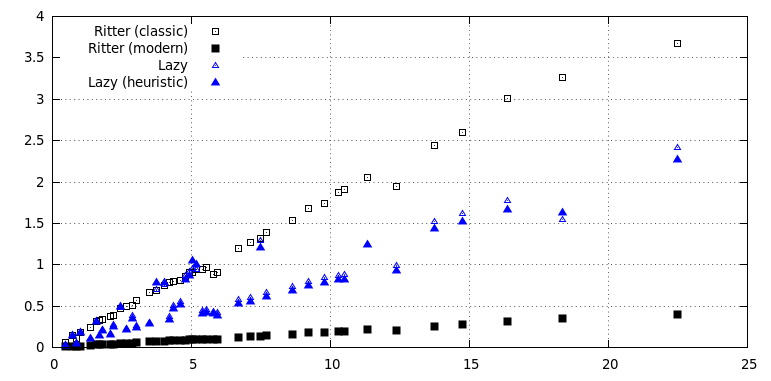
\includegraphics[width=1\linewidth]{image/Rebalances.png}}
	    \caption{Вращения для ДНК}
	\end{figure}
\end{frame}

\begin{frame}
	\begin{figure}[!h]
	    \center{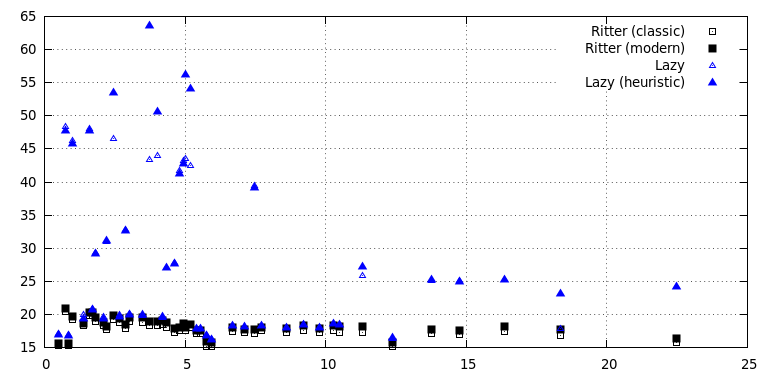
\includegraphics[width=1\linewidth]{image/Ratio.png}}
	    \caption{Степень сжатия для ДНК}
	\end{figure}
\end{frame}

\begin{frame}
	\begin{figure}[!h]
    \center{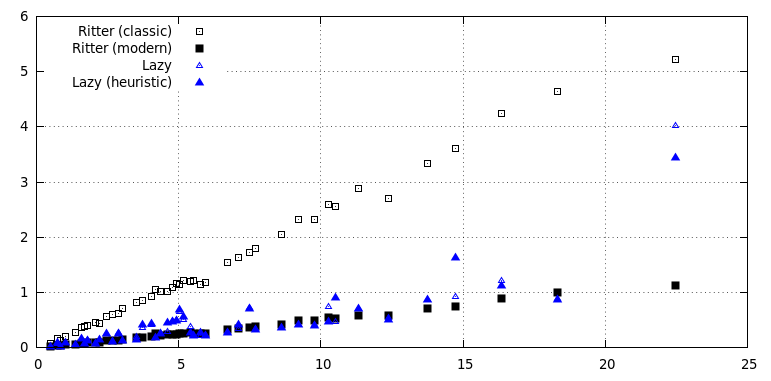
\includegraphics[width=1\linewidth]{image/Time.png}}
    \caption{Время построения для ДНК}
	\end{figure}
\end{frame}

\section{Дальнейшее развитие}

\begin{frame}
\begin{itemize}
  \item Распараллелить.
\pause
  \item Найти среднюю оценку.
\end{itemize}
\end{frame}

\section{Вопросы}

\begin{frame}

	\center{Спасибо за внимание.}
	
	\center{voron13e02@gmail.com}
	\begin{figure}[h]
		\center{
\includegraphics[width=0.2\linewidth]{image/qr_code.jpg}}
	\label{ris:image}
\end{figure}

\center{http://code.google.com/p/overclocking/}

\end{frame}

\end{document}

\end{document}
